\documentclass[Main]{subfiles}
\begin{document}


%NUMBERING of all subsubsection ecc (in order to better grasp the quantization procedure scheme)
\setcounter{secnumdepth}{5} % seting level of numbering (default for "report" is 3). With ''-1'' you have non number also for chapters
\renewcommand\thesubsubsection{\Alph{subsubsection}}
\renewcommand\theparagraph{\thesubsubsection.\alph{paragraph}}
\renewcommand\thesubparagraph{\theparagraph.\Roman{subparagraph}}

\chapter{Geodesic Fields}
	%mettere nell'intro una breve introduzione al problema geodetico nell'approccio standard della geometria riemmaniana
	In the context of differential geometry, \emph{geodesic curves} are a generalization of \emph{straight lines}  in the sense of self-parallel curves.\\
	%Definizione di geodetica su varietà con connessione
	Considering a differential manifold $M$ endowed with an affine connection $\nabla$ we define:
	\begin{definition}[Geodesic]
		A smooth curve $\gamma:[a,b]\rightarrow M$ such that:
		\begin{equation}
			\nabla_{\dot{\gamma}}\dot{\gamma} =0
		\end{equation}
		where $\dot{\gamma}^\mu \coloneqq \frac{d \gamma^\mu}{d t}$ is the tangent vector to the curve.
	\end{definition}
	

		In local chart the previous equation assumes the well-known expression:
		\begin{equation}\label{GeodesicEquation}
			\ddot{\gamma}^i + \Gamma^i_{\, j k} \dot{\gamma}^j \dot{\gamma}^k = 0
		\end{equation}
		where $ \Gamma^i_{\, j k}$ is the coordinate representation of the Christoffel symbols of the connection.
		
		Equation (\ref{GeodesicEquation}) admits a well-posed Cauchy problem.
		\begin{theorem}
			Let $M$ be a smooth manifold, $p\in M$, $v \in T_p M$. 
			Then there exist $\epsilon>0$ and precisely one geodesic
			\begin{displaymath}
				c: [0,\epsilon]\rightarrow M
			\end{displaymath}
			with $c(0) = p , \dot{c}(0) = v$.\\
			 In addition, $c$ depends smoothly on $p$ and $v$.
		\end{theorem}
		\begin{proof}
		Equation \ref{GeodesicEquation} is a system of second order ODE, and the Picard-Lindelof theorem yields the local existence and uniqueness of a solution with prescribed initial values and derivatives, and this solution depends smoothly on the data.
		\end{proof}

	\vspace{4mm}
	%Definizione metrica di geodetica su varietà riemmaniana( con connessione di levi civita)	
	In presence of a pseudo-Riemannian metric it is possible to present the geodesic %in a metric sense i.e. 
	as the curve extremizing the \emph{energy Functional}\footnote{Remember that for arc-length parametrized curves the Energy functional coincides with the length functional.\cite[Lemma $1.4.2$ ]{Jost2005}}:
	\begin{definition}[Energy functional]
  	\begin{equation}\label{EnergyFunctional}
  		H: C^1\left(\left[a,b\right],Q\right) \rightarrow \Real \qquad
 		H(\gamma) \coloneqq \int_a^b \left\Vert \frac{d \gamma}{dt} (t)\right\Vert^2 dt
 	\end{equation}
\end{definition} 	
	Considering only the proper variations (that keep the end-point fixed), the extremum condition corresponds to equation \ref{GeodesicEquation} where $\nabla$ is the unique Levi-Civita connection (torsion-free and metric-compatible).\cite{Jost2005}

	\vspace{4mm}
		%Problema di Jacobi, deviazione geodetica e legame alla curvatura
	In general relativity the problem of the 
	linearization of the geodesic equation yields the Jacobi equation which takes
	%geodesic equation linearization, named \emph{Jacobi equations} takes
	 a central role. \footnote{Usually in this context takes the name of \emph{Geodesic deviation} problem\cite[pag. 46]{Wald1984} inasmuch Jacobi field describes the difference between the geodesic and an "infinitesimally close" geodesic.}
	
	\begin{definition}[Jacobi Field]
	We call a \emph{Jacobi field} along the geodesic $\gamma$ the tangent vector field over the submanifold $\gamma(t,\tau)$, determined by  a smooth one parameter family of geodesics $ \gamma_\tau$ ( with $\gamma_0=\gamma$), in respect to the $\tau$ coordinate. \textit{i.e.}:
	\begin{displaymath}
	 J = \left. \frac{\partial \gamma_\tau (t)}{\partial \tau}\right\rvert_{\tau=0}
	\end{displaymath}
	\end{definition}
	
		In local charts, a Jacobi field along the geodesic $\gamma$ is solution of a linear ODE:
		\begin{equation}\label{JacobiEquationComponents}
			\big( X''\big)^\mu + R^\mu_{i \alpha \j} T^i X^\alpha T^j =0
		\end{equation}
		where:
		\begin{itemize}
			\item $\big(X'\big)^\mu \coloneqq \big( \nabla_{\dot{\gamma}(t)} X\big)^\mu$ is the covariant derivative along the curve $\gamma$.
			\item $T \equiv \dot{\gamma}(t)$ stands for the tangent vector to $\gamma$.
			\item $R^\mu_{i \alpha \j}$ are the representation in components of the Riemann curvature tensor,
		\end{itemize}

	
	
	
	
	The rest of this chapter will be devoted to discussing geodesic and Jacobi fields
	% the presentation of the approach to geodesic and Jacobi problem 
	as a physical system.


\section{Geodesic Problem as a Mechanical Systems}\label{GeodesicMechanics}
	% Da quanto detto in introduzione ha un odore molto forte il legame  dell'equazione geodetica con l'equazione del moto di un punto su una varietà e dell' funzionale lunghezza come versione con il prinicpio di minima azione
	The basic idea is very simple, to portray the geodesic curve as the natural motion of a free point particle constrained on the Pseudo-Riemannian manifold $Q$.
	
	\begin{remark}
	In terms of general relativity this problem can be instantly recognized as the derivation of the motion of free-falling particles.
	
	However, there is no lack of alternative viewpoints .
	The framework of the classical \emph{geometric mechanics} taught us to picture the "static" configurations of a constrained, complex, classical system as a point on the \emph{Configuration space}.% manifold. 
	According to that, the geodesic motion can be seen as a realization of a particular dynamics on a mechanical system with a pseudo-Riemannian configuration space\footnote{Such systems can be depicted as "geodesic" even in presence of a position-dependant potential.\cite[Cap 3.7]{Abraham1978}}.
	\end{remark}


	% Q è la varietà riemmanian in esame, eccc. vedi pag 223  e successive del fomm (direi di dare per assodato tutto il contesto di meccanica geometrica che mi sono studiato nei primi mesi della tesi ma credo non sia il caso di mettere per esteso qui, al massimo solo linkarlo

	\begin{proposition}[Geodesic Motion]
		The geodesics on the Pseudo-Riemannian manifold $(Q,g)$ are the natural motions of the ordinary Lagrangian system $(Q, L)$ where:
		\begin{equation}
			L(V_q) \coloneqq \frac{1}{2} g_q(V,V)
		\end{equation}
	\end{proposition}	
	\begin{proof}
		%	 The Euler-Lagrange equation of $L$ coincides with the geodesic equation \ref{GeodesicEquation}.
		%	 \danger.. è sul quaderno non so se metterla (ho dovuto staccare i foglio per portarmeli a lecce!) ora sono pinzati al quanderno 2
		A direct computation of the Euler-Lagrange equations:
		\begin{displaymath}
			\frac{d}{dt} \left( \frac{\partial L}{\partial V^i}\right) = \frac{\partial L}{\partial q^i}
		\end{displaymath}
		for the Lagrangian
		\begin{displaymath}
			L = \frac{1}{2} g_{i j} ( \vec{q} ) V^i V^j
		\end{displaymath}
		brings to the following equation motion:
		\begin{displaymath}
			g_{k j} \ddot{q}^j = \left(
				 \frac{1}{2} \left(
				 	\frac{\partial g_{i j}}{\partial q^k} \dot{q}^i \dot{q}^j \right)
				  - \frac{\partial g_{k j}}{\partial q^i} \dot{q}^i \dot{q}^j  \right)
		\end{displaymath}
		Multiplying for the inverse of the metric we find:
		\begin{displaymath}
			g^{l k} g_{k j } \ddot{q}^j \equiv \ddot{q}^l = \frac{1}{2} g^{l k} \left( \frac{\partial g_{i j}}{\partial q^k} - \frac{\partial g_{k j}}{\partial q^i}- \frac{\partial g_{k i}}{\partial q^j}\right) \dot{q}^i \dot{q}^j 
			= - \Gamma^l_{\, i j} \dot{q}^i \dot{q}^j
		\end{displaymath}
		where in the last equation we have recognized the expression of Christoffel symbols in term of the Riemannian metric.
	\end{proof}

%	\begin{observation}
	\begin{remark}
		The geodesic system is not simply Lagrangian but also Hamiltonian.
		This property follows from the hyperregularity\cite{Abraham1978} of $L$.
	\end{remark}
%	\end{observation}

	%Qualsiasi sistema di mqo come il precedente può essere visto come un sistema campo.
	As shown in chapter 2, every system with discrete degrees of freedom can be seen as a trivial field system.
	From that it follows the alternative characterization of geodesics as a Lagrangian field:
	\begin{corollary}[Geodesic field]
		The geodesics on the Pseudo-Riemannian manifold $(Q,g)$ can be seen as the \emph{Dynamical Configurations} of the Lagrangian field system $(E,\Lagrangian)$ where:
		\begin{itemize}
			\item $E=(Q\times\Real, \pi, \Real)$ trivial smooth bundle on the real line.
			\item $\Lagrangian[\gamma] = \frac{1}{2} g(\dot{\gamma},\dot{\gamma})(t) dt$
		\end{itemize}
	\end{corollary}
	\begin{proof}
		It is a simple application of the correspondence seen in chapter \ref{MechanicsAsAField}.
	\end{proof}
	
	From this perspective it is clear that the energy functional corresponds to the action of the geodesic field dynamics and equation \ref{GeodesicEquation} is nothing more than the equations of motion according to the \emph{least action principle}.

% \danger aggiungere!!!
%		\begin{figure}[h!]
%		 \centering
   	%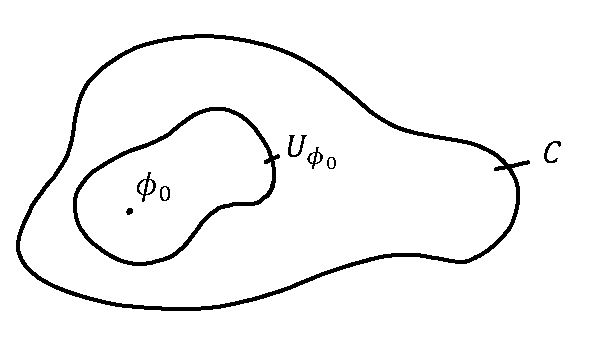
\includegraphics[width=0.5\textwidth]{Pictures/Linearization} 
   	% (credo sia la figura pagina 1 del quaderno 2)
%	 	 \caption{Impressionistic view of the geometric mechanics structure.}
%		\end{figure}		


\section{Peierls Bracket of the Geodesic field}
	The local coordinate expression for the Lagrangian density of the geodesic field is:
	\begin{equation}
		\Lagrangian\big(t,\gamma^i(t), \dot{\gamma}^i(t) \big)\coloneqq \frac{1}{2}g_{\mu,\nu}\left(\gamma^i\left(t\right)\right)\dot{\gamma}^\mu \dot{\gamma}^\nu
	\end{equation}		
	which is highly non-linear. \\
	It is explicitly is quadratic in the velocity components $\dot{\gamma}^i$ and implicitly, through $g_{\mu\nu}(\gamma^i(t))$, is non-polynomial in the %curve 
	coordinates $\gamma^i$.
	
	As show in section \ref{Section:NonLinearPeierls}, for this type of systems the calculation of the Peierls bracket can be realized only locally around a predetermined solution.\\
	Let us repeat the Peierls' procedure for the system under investigation.

	As a consequence of our introduction on the geodesic as a field, we can state the unperturbed dynamic as a L.P.D.O :
		\begin{equation}
			Q_\Lagrangian \big(q^\mu 	\big)= \biggr[\ddot{q}^\mu + \Gamma^\mu_{\, i j}\dot{q}^i \dot{q}^j	\biggr]
		\end{equation}
	where $\dot{q}^\mu = \frac{d}{dt}q^\mu(t)=\dot{q}^i\partial_i q^\mu$.
	
	A linear variation of $q_0^\mu +\epsilon \eta^\mu$ constructed from the coordinate representation $q_0^\mu$ of the geodesic $\gamma_0 \in \Sol$, solves the original equations of motion when
	\begin{equation}\label{GeodesicJacobation1}
		Q_\Lagrangian \big( q_0^\mu +\epsilon \eta^\mu \big) = \frac{d^2}{dt^2}\biggr( q_0^\mu +\epsilon \eta^\mu \biggr) +
		\biggr[ \Gamma^\mu_{\, i j}\big( \vec{q_0} + \epsilon \vec{\eta}\big) \biggr]\biggr(\dot{q_0}^i +\epsilon \dot{\eta}^i \biggr)\biggr(\dot{q_0}^j +\epsilon \dot{\eta}^j \biggr) = 0 \mbeq o(\epsilon)
	\end{equation}
	If we consider only the first order in the parameter $\epsilon$ we can expand the expression of the Christoffel symbols:
	\begin{displaymath}
		\biggr[ \Gamma^\mu_{\, i j}\big( \vec{q_0} + \epsilon \vec{\eta}\big) \biggr] =
		\biggr[ \Gamma^\mu_{\, i j}( \vec{q_0}) + \epsilon \eta^\alpha\big( \partial_\alpha  \Gamma^\mu_{\, i j} \big)\biggr\vert_{\vec{q_0}} + o(\epsilon) \biggr]
	\end{displaymath}	 
	
	Collecting all the terms in equation \ref{GeodesicJacobation1} up to the first order in $\epsilon$ it follows a condition on the perturbation:
	\begin{align}\label{Eq:JacobiPeierlsEquation}
	0 &= \ddot{\eta}^\mu + \eta^\alpha\big( \partial_\alpha  \Gamma^\mu_{\, i j} \big)\biggr\vert_{\vec{q_0}} \dot{q_0}^i \dot{q_0}^j  +  \Gamma^\mu_{\, i j} \big(\dot{\eta}^i \dot{q_0}^j + \dot{q_0}^i \dot{\eta}^j \big)= \nonumber \\
	&=\biggr\{ g^\mu_{\,\alpha} \frac{d^2}{dt^2} +
	 \Gamma^\mu_{\, i \alpha}(\vec{q_0})\big[2 \dot{q_0}^i \frac{d}{dt} \big] + 
\big[ \partial_\alpha \Gamma^\mu_{\, i j}(\vec{q_0}) \dot{q_0}^i \dot{q_0}^j  \big] \biggr\} \eta^\alpha	= P^\mu_{\: \alpha} \eta^\alpha
	\end{align}		
	where $ P^\mu_{\: \alpha}$ is a linear partial differential operator acting on the \emph{variations} \textit{,i.e.,} the components of a field along the geodesic $\gamma_0$.\\
	As showed in section \ref{Section:NonLinearPeierls}, equating the linearized dynamics operator with the term $-\left(Q_\chi(\gamma_0)\right)(x)$ 	(see equation \ref{PeierlJacobiEqNonLin}) leads to the inhomogeneous \emph{Jacobi operator} from which all the standard construction of the brackets Peierls follows.

	
	\begin{proposition}
		The differential equation $$P^\mu_{\: \alpha} \eta^\alpha=0$$ corresponding to the l.p.d.o. $P$ defined in equation \ref{GeodesicJacobation1} corresponds to equation \ref{JacobiEquationComponents} defining  the \emph{Jacobi fields} along the geodesic $\gamma_0$.
	\end{proposition}
	\begin{proof}
		For convenience, we adopt the following notation:
		\begin{align*}
		&\eta^\mu \partial_\mu \coloneqq X \equiv X^\mu \partial_\mu \\
		&\dot{q_0}^i \partial_i \equiv \dot{\gamma_0} \coloneqq T \equiv T^i \partial_i
		\end{align*}
		We have to show that the equation just found:
		\begin{equation}\label{JacobiEqI}
			\ddot{X}^\mu + X^\alpha\left(\partial_\alpha\Gamma^{\mu}_{\, i j}\right)T^i T^j + \Gamma^\mu_{\, \alpha j}\left(2 T^j \dot{X}^\alpha \right) = 0
		\end{equation}
		where $\dot{X}^\mu = \frac{d}{dt}X^\mu= T^i \partial_i X^\mu$,
		corresponds to the equation defying the Jacobi field:
		\begin{equation}\label{JacobiEqII}
			\left(X'' \right)^\mu + R^\mu_{\, i \alpha j}T^i X^\alpha T^j = 0
		\end{equation}
		where $\left(X')\right)^\mu \coloneqq \left(D_t X \right)^\mu$ and $D_t = T^i \nabla_i$ is the covariant derivative along the curve.\\
		Since:
		\begin{align}\label{JacobiEqDerivative}
			X'' &= D_t D_t X = D_t \left( \partial_\mu \left( \dot{X}^\mu + \Gamma^\mu_{\, i \alpha} T^i X^\alpha \right)\right) \nonumber \\
			&=\left( \ddot{X}^\mu + \frac{d}{dt}\left( \Gamma^\mu_{\, j \alpha} T^j X^\alpha \right) + \Gamma^\mu_{\, j \nu}T^j \dot{X}^\nu + T^j \Gamma^\mu_{\, j \nu} \Gamma^\nu_{\, i \alpha} T^i X^\alpha \right)\partial_\mu
		\end{align}
		We can write equation \ref{JacobiEqI} in term of the covariant derivative as:
		\begin{align*}
			\left(X'' \right)^\mu &=
			- \left(
			X^\alpha\left(\partial_\alpha\Gamma^{\mu}_{\, i j}\right)T^i T^j + \Gamma^\mu_{\, \alpha i}\left(2 T^i \dot{X}^\alpha \right)
			- \frac{d}{dt}\left( \Gamma^\mu_{i \alpha} T^i X^\alpha \right) - T^j \Gamma^\mu_{\, j s} \Gamma^s_{\, i \alpha} T^i X^\alpha
			\right) =\\
			&=			
			-\left(
			X^\alpha\left(\partial_\alpha\Gamma^{\mu}_{\, i j}\right)T^i T^j - \dot{\Gamma}^\mu_{i \alpha} T^i X^\alpha
			- \Gamma^\mu_{i \alpha} \dot{T}^i X^\alpha  - T^j \Gamma^\mu_{\, j s} \Gamma^s_{\, i \alpha} T^i X^\alpha				
			\right)
		\end{align*}
		remembering that the geodesic condition is still to be met:
		\begin{displaymath}
			\dot{T}^i = - \Gamma^I_{\, j k} T^j T^k
		\end{displaymath}
		we can conclude that:
		\begin{align*}
			\left(X'' \right)^\mu &=
			- \left(
			  X^\alpha\left( \partial_\alpha\Gamma^\mu_{\, i j}\right)T^i T^j
			- T^j \left( \partial_j \Gamma^\mu_{\, i \alpha}\right) T^i X^\alpha
			+X^\alpha \Gamma^\mu_{\, \alpha s} \Gamma^s_{\, i j}T^i T^j 
			- T^j \Gamma^\mu_{\, j s} \Gamma^s_{\, i \alpha} T^i X^\alpha
			\right) =\\
			&=	-\left( R^\mu_{\, i \alpha j}T^i X^\alpha T^j\right)		
		\end{align*}
	\end{proof}
	
	

	
	

\subsection{Example: Geodesic field on FRW spacetime}
\ifToninus
	\begin{Warning}
	% qui i conti li devo ancora fare, 
	l'idea è che per scelta di metrica e geodetica semplici le equazioni di jacobi possono essere disaccoppiate a dare 4 ode di cui in linea di principio posso calcolare la funzione di green	

	\vspace{2mm}
	Per Ripasso di FRW: \url{http://universeinproblems.com/index.php/Friedman-Lemaitre-Robertson-Walker_(FLRW)_metric#Problem_1:_expanding_baloon}

	\vspace{2mm}
	L'esempio deve articolarsi così:
		\begin{enumerate}
			\item Introdurre la Metrica FRW come fa CD (ricordare che è GH)
			\item Calcolo Cristoffel (uso Mathematica)
			\item Equazione Geodetica
			\item Calcolo R
			\item Do espressione in coordinate per il campo di Jacobi
			\item Verifico che trovo 4 equazioni Disaccoppiate (credo che sarà necessario mettersi nelle coordinate che dice Wiki)
			\item calcolo le 2 soluzioni omogenee per ogni componente
			\item ricordare cos'è l'operatore di green in generale, se l'op è diagonale ricordare come si semplifica (cioè ho 4 op di green per ogni ode), ricordare cos'è l'op di green per una ODE (cioè operatore  a nucleo integrale, il nucleo è detto 
			\item Criterio per il calcolo delle green per delle ODE lineari di secondo ordine
			\item realizzo il calcolo per ogni componente di jacobi
			\item realizzo l'op di green (dovrebbe dipendere dalla geodetica da cui sono partito ) è dico come va inserito per ottenere il disturbo
			\item limitandosi al caso di densità lagrangiane lineari trovo il disturbo e le peierls
		\end{enumerate}
	\end{Warning}
\fi	
	Let us compute the Peierls' bracket for the single special case of geodesic motion on Friedmann–Lemaître–Robertson–Walker spacetimes (FRW).
	
	We recall that the FRW spacetimes are homogeneous and isotropic solutions of Einstein's equations.
	These manifolds are endowed with a line element of the form:
	\begin{equation}\label{EQ: metrica FRW}
		ds^2 = -dt^2 + a^2(t) \left( \frac{dr^2}{1-k r^2} + r^2 d\theta^2 + sin^2\theta d\phi^2\right)
	\end{equation}
		where $0 < a(t) \in C^\infty	(I)$ is said \emph{scale factor}, $I \subset \Real$ is the time domain and $k$ is a constant normalizable to $\pm 1$ or $0$.\\
		The assumptions of homogeneity and isotropy alone determine the spacetime metric up to the value of the scale factor $a$ and up to three possibilities of spatial geometry.
		The simply connected spacetimes compatibile with \ref{EQ: metrica FRW} are topologically equivalent (diffeomorphic) 		
		to $\Real \times \Sigma$ where $\Sigma$ is a 3D manifold which depends on the value of $k$:
		\begin{center}\begin{tabular}{l l}
			$k = 1$ & $\Sigma \simeq S^3$ (3-sphere)\\
			$k = 0$ & $\Sigma \simeq \Real^3$ (three-dimensional Euclidean space)\\
			$k = -1$ & $\Sigma \simeq H^3$ ( three-dimensional hyperboloid)\\		
		\end{tabular}\end{center}
		\vspace{2mm}
\ifToninus
		\begin{Warning}
		CD:
		\emph{veramente sono equivalenti come varietà differenziabile e non solo topologica}
		\end{Warning}
\fi

		For the sake of simplicity let us reduce ourselves to the case of \emph{flat} spatial geometry, \textit{i.e.}:
		\begin{displaymath}
			ds^2 = -dt^2 + a^2(t) \left( dx^2 + dy^2 + dz^2\right) = g_{\mu \nu} dx^\mu dx^\nu
		\end{displaymath}
		in the \emph{cosmological} reference frame.
\ifToninus
	\begin{Warning}
		Una possibile giustificazione a questa tesi è : evidenze sperimentali in ambito cosmologico suggeriscono che $k=0$
	\end{Warning}
\fi


		In order to write explicitly the geodesic equation we have to compute the Christoffel symbols. According to the basic definition:
		\begin{displaymath}
			\Gamma^\lambda_{\, \mu \nu} = \frac{1}{2} g^{\lambda \sigma } \left( \partial_\mu g_{\sigma \nu} + \partial_\nu g_{\mu \sigma} - \partial_{\sigma}g_{\mu \nu} \right)
		\end{displaymath}
		we find that the non-vanishing components of $\Gamma^\lambda_{\, \mu \nu}$ are : %merely:
			\begin{align}
				\Gamma^0_{\, i i} &= a \dot{a} \\
				\Gamma^i_{\, i 0} &= \Gamma^i_{\, 0 i} = \dfrac{\dot{a}}{a}
			\end{align}
			where we have used the usual convention to express with latin indices the spatial coordinates, with $0$ the time coordinate and with Greek indices all the spacetime coordinates.
			
			In the cosmological coordinate chart the geodesic equation reads:
			\begin{eqnarray}
				\frac{d^2}{d \tau^2} \gamma^0 &= - a \dot{a} \left( \frac{d}{d \tau} \gamma^i \frac{d}{d \tau}\gamma_i \right) \label{FRWGeo1}\\
				\frac{d^2}{d \tau^2} \gamma^i &= - 2 \dfrac{\dot{a}}{a} \left( \frac{d}{d \tau} \gamma^0 \frac{d}{d \tau}\gamma^i \right) 		\label{FRWGeo2}	
			\end{eqnarray}
			
			Jacobi fields are dependant on the choice of a base geodesic. 
			Let us consider a simple time-like geodesic, namely the \emph{cosmological} free-falling observer:
			\begin{displaymath}
				\gamma^\mu (t) = \begin{bmatrix}  a_0 + m t \\  a_1 \\ a_2 \\ a_3  \end{bmatrix}
				\qquad
				T^\mu=\frac{d}{d t}\gamma^\mu(t)= \begin{bmatrix}  m \\  0 \\ 0 \\ 0  \end{bmatrix}
			\end{displaymath}
\ifToninus
	\begin{Warning}
		Sul quaderno ho scritto un po' di più rifacendomi al discorso visto su wiki Jacobi Fields.
	\end{Warning}
\fi
			Remembering the definition of the components of the Riemann tensor:
			\begin{displaymath}
				{R^\sigma}_{\mu\nu\kappa} =
				  {\partial{\Gamma^\sigma}_{\mu\nu} \over \partial x^\kappa} -
				  {\partial{\Gamma^\sigma}_{\mu\kappa} \over \partial x^\nu} +
				  {\Gamma^\lambda}_{\mu\nu}{\Gamma^\sigma}_{\kappa\lambda} -
				  {\Gamma^\lambda}_{\mu\kappa}{\Gamma^\sigma}_{\nu\lambda}		
			\end{displaymath}			 
			we find by direct computation  that the non vanishing components are:
			\begin{equation}
				R^0_{\: i 0 i}= - R^{0}_{\: i i 0}= a \ddot{a} \qquad
				R^i_{\: 0 0 i}=-R^i_{\: 0 i 0}=	\dfrac{\ddot{a}}{a}\qquad
				R^i_{\: j i j} = - R^i_{\: j j i} = \dot{a}^2				
			\end{equation}
			Since we have parametrized the curve with $x^0 = t$ the covariant derivative in Eq. \ref{JacobiEquationComponents}  corresponds to an ordinary derivative, then a Jacobi $X^\mu(t)$ along the time-like geodesic $\gamma(t)$ satisfies the following uncoupled homogeneous equations:
			\begin{eqnarray}
				\frac{d^2}{d t^2} X^0  &=& 0 \label{FRWJacobi1}\\
				\frac{d^2}{d t^2} X^i &= &- m^2 R^{\mu}_{\: 0 \nu 0} X^\nu = \left( m^2 \frac{\ddot{a}}{a}\right) X^i 	\label{FRWJacobi2}	
			\end{eqnarray}			
			\vspace{2mm}
			
			Regarding this problem as a field system, we can say that the operator $P$ ruling the dynamics is diagonal:
			\begin{displaymath}
				P X =
				 \begin{bmatrix}  
				 \left(\frac{d}{dt}\right)^2 & 0 \\
				 0 & \IdOp \left( \left(\frac{d}{dt}\right)^2 - m^2 \frac{\ddot{a}}{a} \right)
				 \end{bmatrix}
				 \begin{bmatrix} X^0 \\ X^i  \end{bmatrix}
				 = 0
			\end{displaymath}
			
			The main difficulty to face in the explicit Peierls bracket construction is the computation of the Green operator of $P$.
			In this case we can say with certainty that both Green operators are diagonal:
			\begin{displaymath}
				G^\pm =
				 \begin{bmatrix}  
				 G^\pm_0 & 0 \\
				 0 & G^\pm_i
				 \end{bmatrix}
			\end{displaymath}		
			where $G^\pm_0$ and $G^\pm_i$ are the Green operators of the only two ODEs involved:
			\begin{displaymath}
				P_0 = \left(\frac{d}{dt}\right)^2 \qquad P_i=\left( \frac{d^2}{dt^2} - m^2 \frac{\ddot{a}}{a} \right)
			\end{displaymath}
			As proved in Section \ref{Section:GreenFunctions} these are  Hilbert–Schmidt integral operators:
			\begin{displaymath}
				G^\pm_\mu f(t) = \int_\Real g^\pm_\mu( t \vert \xi ) f(\xi) d\xi
			\end{displaymath}
			where the integral kernel function is given by  Equation \ref{Eq:AdvRetGreenFunction}.
			
			Eq. \ref{FRWJacobi1} is a linear autonomous ordinary differential equation, two explicit linearly independent solutions are 
			\begin{displaymath}
				\varphi_1(x)=1 \qquad \varphi_2(t)=t
			\end{displaymath} 
			with $W(1,t)=1$. \\
			The advanced and retarded Green functions corresponding to $P_0$ can be promptly computed:
			\begin{equation}\label{SimpleGreenFunction}
				g^\pm_0(t \vert \xi) = \pm \theta\big(\pm(t-\xi)\big) \left[ t -\xi\right]
			\end{equation}
			
			At the same time, since the coefficient $m^2 \frac{\ddot{a}(t)}{a(t)}$ is in general time dependant,  Eq. \ref{FRWJacobi2} is a non autonomous ODE and an analytical expression of its general solution does not exist.
\ifToninus
	\begin{Warning}	
		Anche un'appendice sul calcolo delle green sfruttando lo sviluppo di Dyson e quello di Magnus ( Partendo come spunto dall'articolo \cite{Dappiaggi2014}) non sarebbe stata male. ma è venuto il tempo di concludere.
	\end{Warning}
\fi	
			\\
			It is possible, however, to express the corresponding Green function as a convergent Dyson expansion\cite{Dappiaggi2014}.
			The idea is to consider the non-autonomous term $V(t) = -m^2 \frac{\ddot{a}(t)}{a(t)}$ as if it were a perturbing potential.\\
			Remembering that $G^\pm_0 (t \vert \xi)$ is the Green function of operator \ifToninus$P_{0}=\left(\frac{d}{dt}\right)^2$\else$P_0$\fi, which can be seen as the time-independent part of differential operator \ifToninus$P_{i i}=\left( \left(\frac{d}{dt}\right)^2 - m^2 \frac{\ddot{a}}{a} \right)$\else$P_i$\fi, we can formally express the Green function of $P_{i}$ as follow:
			
			\begin{align*}
				G^+_i ( \tau \vert \tau' ) = G^+_0( \tau \vert \tau' ) + \sum_{n=1}^\infty (-)^n 
				\int_{-\infty}^\tau dt_1 \cdots \int_{-\infty}^{t_{n-1}} dt_{n-1} 
				& \,  G^+_0(\tau \vert t_1) G^+_0(t_1\vert t_2) \cdots G^+_0(t_{n-1} \vert t_n) \times \\
				& \times  V(t_1) V(t_2) \cdots V(t_n) \times \\
				& \times  G^+_0 (t_n \vert \tau' ) \\
			\end{align*}		
			similarly $G^-_i$  can be obtained considering the advanced Green function $G^-_0$ and integrating from $t$ to $+\infty$.
			In both cases the convergence of the series is not guaranteed and should be verified for each explicit expression of the scale function $a (t)$.
			
			\vspace{2mm}
			\ifToninus Anyway all this machinery it is not necessary \fi In the special case of \emph{De Sitter} spacetime, where $ a(t) = \exp(H t)$ and the coefficient $\ddot{a}/a=H^2$ is a positive constant  \cite{Wald1984}, 
			two linearly independent solutions are given by
			\begin{displaymath}
				\varphi_1(x) = e^{-V t} \qquad \varphi_2(x)= e^{Vt}
			\end{displaymath}
			with $V=m H$ and Wronskian $W= 2V$.
			The Green functions are
			\begin{displaymath}
								g^\pm_i(t \vert \xi) = \pm \frac{1}{2V}\theta\big(\pm(t-\xi)\big) \left[ e^{V(t-\xi)} - e^{-V(t-\xi)}\right]
			\end{displaymath}

			Combing all these results we are able to give an explicit expression of the Peierls symplectic form $\tau$- as defined in Eq. 	\ref{Def:SymplecticTau} for the De Sitter spacetime.
			For any pair $(X, Y)$ of compactly supported fields over $\gamma(t)$ we have:
			\begin{align*}
			\{X ,Y \} =&\int \left\langle X, \left(\GreenAdv - \GreenRet \right)Y \right\rangle dt =	\\
			=&
			\int_\Real dt  
				 \begin{bmatrix}  
					 X^0(t) & \vec{X}(t) \\
				 \end{bmatrix}
				 \begin{bmatrix}  
				 	-1 & 0 \\
				 	0 & a^2(t)\IdOp
				 \end{bmatrix}			
				 \begin{bmatrix}  
				 	(G^-_0 - G^+_0) & 0 \\
				 	0 & (G^-_i - G^+_i)
				 \end{bmatrix}	
				 \begin{bmatrix}  
				 	Y^0(t) \\ \vec{Y}(t)
				 \end{bmatrix}	
				 = \\
			=&
				\int_\Real dt  \left(
					-X^0(t) (G^-_0 - G^+_0)Y^0(t)+
					a^2(t)\vec{X} \cdot (G^-_i- G^+_i)\vec{Y}(t)
				\right) = \\
			=&
				\int_\Real dt 				\int_\Real d\xi \left(
					-X^0(t)Y^0(\xi)\big(-\theta(\xi -t)-\theta(t-\xi )\big)\left[t-\xi \right] \right) +\\
			&+
					\int_\Real dt 				\int_\Real d\xi a^2(t) \left(
					\vec{X}(t) \cdot \vec{Y}(\xi)
						\big(-\theta(\xi -t)-\theta(t-\xi )\big) \frac{1}{2V}\left[ e^{V(t-\xi)} - e^{-V(t-\xi)}\right]
					\right) = \\
			=& \int_\Real dt 				\int_\Real d\xi \left(
				X^0(t)Y^0(\xi)\left[t-\xi \right]				-
				\vec{X}(t) \cdot \vec{Y}(\xi) \frac{a^2(t)}{2V}\left[ e^{V(t-\xi)} - e^{-V(t-\xi)}\right]
				\right)
			\end{align*}					
		

\section{Algebraic quantization of the Geodesic Field}
	The algebraic quantization scheme applies only to %linear field systems.
	systems of linear fields.
	Since equation\ref{GeodesicEquation} is highly non linear,  it is not the geodesic system that can actually be quantized but rather its linearization, the Jacobi field along a fixed geodesic $\gamma_0$.
	
		\subsubsection{Classical Framework}
			The basic idea is that, chosen a geodesic $\gamma_0$, the kinematical configurations of the Jacobi fields are tangent fields along the fixed curves.
			\paragraph{Kinematics}	
			The configuration bundle $E$ corresponds to the \emph{Pull-back bundle} $\gamma_0^*(TQ)$ of the tangent bundle along the geodesic $\gamma_0$.
			Then:
			\begin{itemize}
				\item $E$ is a vector bundle over $\Real$.
				\item The base manifold $\Real$ can be considered as a degenerate globally hyperbolic spacetime, $\CauchyClass(\Real) = \Real$.
				\item the fibers are $E_p \coloneqq T_{\gamma_0(p)}Q$
				\item $\Conf = \Gamma^\infty(E) = \mathfrak{X}(\gamma_0)$ is constituted by vector fields along the curve $\gamma_0$.
			\end{itemize}
			
			\paragraph{Dynamics}
				The coordinate representation of the motion equation is:
				\begin{displaymath}
					\left( P X \right)^\mu = (X'')^\mu + R^\mu_{\, i \alpha j } T^i T^j X^\alpha
				\end{displaymath}
				where $X\in \Conf$ and $T^i = \dot{\gamma_0}^i$.
				According to equation \ref{Eq:NormallyHyperbolicRepresentation} this operator falls exactly in the class of \emph{normally hyperbolic} operators hence it is quantizable both by  means of Peierls procedure and by means of initial data.
		
		\subsection{PreQuantum Framework}
		\subsubsection{Peierls approach}
			\paragraph{Pairing}
				%The choice of the inner product on this configuration bundle is rather obvious.
				Since $Q$ is a Riemannian manifold and $\Conf$ is composed by tangent vector fields, it is straightforward to choose as inner product on the configuration bundle $E$ the metric function defined on $Q$:
				\begin{equation}
					\left\langle X,Y \right\rangle_t \coloneqq g\left( X\left(\gamma_0(t) \right),Y\left(\gamma_0(t) \right)\right)
					\qquad \forall X,Y \in E_t
				\end{equation}
				
				It follows slavishly the definition of a pairing:
				\begin{equation}
					\left( X, Y \right) = \int_\Real \left\langle X,Y \right\rangle_t dt
				\end{equation}
				well-defined for every pair $X,Y \in \Conf$ such that $\supp(X) \cap \supp(Y)$ is compact.
				
				The operator $P$ ruling the dynamics is formally self-adjoint:
				\begin{align*}
				 ( Y, PX) &= \int Y_\mu PX^\mu dt= 
				 \int\left( Y_\mu \ddot{X}^\mu + Y_\mu R^\mu_{\, i \alpha j}T^i T^j X^\alpha \right)dt = \\
 				 &= \int\left( \ddot{Y}_\mu X^\mu + X_\mu R^\mu_{\, i \alpha j}T^i T^j Y^\alpha \right)dt =
				 \int P Y_\mu X^\mu dt=( PY, X) 				 				 
				\end{align*}
				where we have integrated by parts twice (the boundary value being null since the integrand is compactly supported) and we have exploited the curvature tensor identity:
				\begin{equation}\label{Eq:CurvatureSimmetry}
					\langle R(X,T)T,Y \rangle = \langle R(Y,T)T,X \rangle
				\end{equation}

			\paragraph{Classical Observables}
				Replicating what has been done in the general case, 
				we construct the \emph{pre-observables} as the functionals $F_f:\Conf \rightarrow \Real$ for all $f \in \Gamma_0(E)$ compactly supported fields along the geodesic $\gamma_0$:
				\begin{equation}
					F_f(X) = \int_\Real <X, f>_t dt \qquad \forall X \in \Conf
				%	F_f(X) = \int_{\dom(\gamma_0)} <X, f>_t dt \qquad \forall X \in \Conf
				\end{equation}
				The space of classical observables is then obtained through the usual quotient:
				\begin{displaymath}
					\Obs \simeq \frac{\Gamma_0}{P \Gamma_0}
				\end{displaymath}
				The observables functionals are the maps:
				\begin{displaymath}
				 F_{[f]}(X) = F_f (X) \qquad \forall X \in \Sol
				\end{displaymath}
				where $f$ is a representative of the equivalence class $[f]\in \Obs$.
			
			\paragraph{Symplectic Structure}
				The geodesic motion is a particular case of a system with finite degrees of freedom, thus the Peierls brackets between two Lagrangian functionals $\chi, \omega$ around a geodesic $\gamma_0$ tested on a function $f \in C_0^\infty(\Real)$ are given by Eq.  \ref{EspressionePeierlsCampiCurve}.\\
				Restricting the definition to the simplest Lagrangian functionals constructible from the classical observables:
				\begin{displaymath}
					\chi [\phi] \coloneqq (\chi, \phi) \qquad \chi \in \Obs,\, \phi \in \Sol
				\end{displaymath}
				corresponding to Lagrangian densities in the form:
				\begin{displaymath}
					\chi ( \vec{q}i, \dot{\vec{q}}) \coloneqq < \chi, \vec{q}> = \chi^i q_i
				\end{displaymath}
				such that $ Q_\chi \gamma_0^i = \chi^i$, the Peierls brackets expression reduces to
				\begin{displaymath}
					\left\lbrace\chi , \omega \right\rbrace (\gamma_0) [f] = \int f(t) \left\langle\chi, \left(\GreenAdv - \GreenRet \right)\omega \right\rangle dt
				\end{displaymath}
				The test-function $f$ can be neglected for regular distributions.
%				For regular distribution can be neglected the test-function $f$.

				\vspace{3.5mm}
				We conclude that,according to the Peierls' procedure,  the classical symplectic space is the pair $(\Obs, \tau)$ where:
				\begin{displaymath}
					\tau( [\chi], [\omega]) = \{\chi , \omega \} =\int \left\langle\chi, \left(\GreenAdv - \GreenRet \right)\omega \right\rangle dt = ( \chi, E \omega) \qquad \forall \chi,\omega \in \Gamma_0(E)
				\end{displaymath}
				
				
		\subsubsection{Initial data Approach}
			\paragraph{Classical Phase Space}
				The base manifold for the configuration bundle under examination is the real line $\Real$ that can be seen as a degenerate globally hyperbolic spacetime.
				Thus each point $p\in \Real$ is a Cauchy surfaces and no further support condition can be imposed.\\
				Considering that the operator $P$ is of second order, we have:
				\begin{displaymath}
					\Phase(p) \equiv \Data(p) = \Gamma^\infty(p) \times \Gamma^\infty(p) =
					T_{\gamma_0(p)}Q \times T_{\gamma_0(p)}Q
				\end{displaymath}
				and
				\begin{displaymath}
					\Phase \simeq \Sol
				\end{displaymath}
				using the map which yields the unique solution starting from an initial data.
				
			\paragraph{Symplectic Structure on the Phase Space}		
				The general definition \ref{Def:InitialDataSymplecticForm} of the symplectic form on the classical phase space reduces to:
				\begin{displaymath}
					\Omega: \Phase(p) \times \Phase(p) \rightarrow \Complex \qquad : \qquad 					
					\Omega \biggr\{ [V_0,V_1] , [W_0, W_1] \biggr\} = g(V_1,W_0)  - g( V_0, W_1) 
				\end{displaymath}
				where $g$ is the inner product on $Q$.
				\\
				This formula can be transferred to the space of solutions:
				\begin{displaymath}
					\sigma_p: \Sol \times \Sol \rightarrow \Complex \qquad : \qquad 					
					\sigma_p \biggr\{X, Y  \biggr\} = \Omega \biggr\{ [Y(t), D_t Y(t)] , [X(t), D_t X(t)] \biggr\}
				\end{displaymath}
				\vspace{3mm}
				Mimicking what has been done in example \ref{Ex:IndipendentPhaseSpace} for the scalar field, the independence of the phase space construction from the particular choice of $p \in \Real$ can be proved.\\
				Taken $X,Y \in \Sol$ two Jacobi fields on $\gamma_0(t)$, a scalar field over $\Real$ can be defined:
				\begin{displaymath}
					J(t) \coloneqq \Omega \biggr\{ [Y(t), D_t Y(t)] , [X(t), D_t X(t)] \biggr\}
					= X^\alpha(t) g_{\alpha \beta} D_t Y^\beta(t) - 
					Y^\alpha(t) g_{\alpha \beta} D_t X^\beta(t) 					
				\end{displaymath}
				where $D_t = T^\mu \nabla_\mu$ as usual.
				This is clearly a conserved current:
				\begin{eqnarray}
					D_t J =& (D_t X)^\alpha g_{\alpha \beta} (D_t Y)^\beta - (D_t Y)^\alpha g_{\alpha \beta} (D_t X)^\alpha + X^\alpha g_{\alpha \beta} D_t D_t Y^\beta - Y^\alpha g_{\alpha \beta} D_t D_t X^\beta = \nonumber \\
					=& X^\alpha g_{\alpha \beta} PY^\beta - Y^\alpha g_{\alpha \beta} PX^\beta - X_\beta R^\beta _{\, i \alpha j}T^i Y^\alpha T^j +Y_\beta R^\beta _{\, i \alpha j}T^i X^\alpha T^j  = 0
				\end{eqnarray}
				exploiting the conditions $\nabla_\mu g_{\alpha \beta}=0$, $PX=PY=0$ and equation \ref{Eq:CurvatureSimmetry}.\\
				Hence:
				\begin{displaymath}
				\int_p^{p'} D_t J = J(p) - J(p') = 0
				\end{displaymath}
			In others words:
			\begin{displaymath}
				\sigma_\Sigma (X, Y) = \sigma_{\Sigma'} (X, Y) 
				\qquad \forall X, Y \in \Sol \; ; \; \forall \Sigma, \Sigma' \in \CauchyClass(M)= \Real
			\end{displaymath}
			
				\vspace{3.5mm}
				In conclusion, according to the initial data procedure,  the classical symplectic space is the pair $(\Sol, \sigma)$ such that:
				\begin{displaymath}
					\sigma( X, Y) = X_\mu(\Sigma) \left( D_t Y (\Sigma)\right)^\nu - \left(D_t X(\Sigma)\right)_\mu Y^\nu(\Sigma) \qquad \forall X,Y \in \Sol
				\end{displaymath}
				where $\Sigma$ is an arbitrary point in $\Real$.

	\subsection{Comparisons}
		The two procedures yield two different classical symplectic spaces: $(\Obs,\tau)$ and $(\Sol, \sigma)$.
		We have proved in section \ref{Section:LinkBetweenQuantization} (Theorem \ref{Teo:IsomorphismBetweenTheTwoSymplectic}) that the two vector spaces are isomorphic through the map $\Xi$ realized with the causal propagator $E$ .
		Furthermore, in this case it can be proved that $\Xi$ preserves the symplectic form.
		
		Once again we mimic what has been done for the case of a scalar field (Ex \ref{Ex:SimplettomorphismPhaseSpace}).\\
		Consider two compactly supported vector fields $f,h \in \Gamma_0(E)$ along $\gamma_0$	and call $X= Ef,\: T = Eh$ the corresponding Jacobi field.
		In fact from the definition of $\tau$ it follows:
		\begin{align}
			\tau\big( [f], [g] \big) =& (f, Eh) = \int_\Real f^\mu g_{\mu \nu} ( E h)^\nu dt =
					\int_\Sigma^\infty  f^\mu g_{\mu \nu} Y^\nu dt	 + 
					\int_{-\infty}^\Sigma  f^\mu g_{\mu \nu} Y^\nu dt
			\nonumber \\
			=& \int_\Sigma^\infty (P \GreenAdv f)^\mu g_{\mu \nu} Y^\nu dt	 + 
					\int_{-\infty}^\Sigma (P \GreenRet f)^\mu g_{\mu \nu} Y^\nu dt
		\end{align}
		where the integral has been decomposed by splitting the domain of integration into two subsets whose intersection has zero measure and we have exploited the properties of the retarded and advanced operators.

		Considering the explicit representation of the operator $P$, we can integrate by parts twice:
		\begin{align}
			&\int_\Sigma^\infty (P \GreenAdv f)^\mu g_{\mu \nu} Y^\nu dt = \int_\Sigma^\infty \left( D_t^{\,2} \GreenAdv f +R(\GreenAdv f,T)T \right)^\mu g_{\mu \nu} Y^\nu dt \quad = \nonumber \\
			&= 
			 \int_\Sigma^\infty D_t \left( \left(D_t  \GreenAdv f \right)^\mu g_{\mu \nu} Y^\nu \right)dt -
			 \int_\Sigma^\infty \left( D_t  \GreenAdv f \right)^\mu g_{\mu \nu} \left( D_t Y \right)^\nu dt \quad + \nonumber \\
			 &\quad + \int_\Sigma^\infty \left( R( \GreenAdv f,T)T \right)^\mu g_{\mu \nu} Y^\nu dt \quad = \nonumber \\
			&= 
			 - \left. D_t( \GreenAdv f)^\mu g_{\mu \nu} Y^\nu \right\vert_\Sigma -
			 \int_\Sigma^\infty D_t \left( \left( \GreenAdv f \right)^\mu g_{\mu \nu} \left( D_t Y \right)^\nu \right)dt \quad + \nonumber \\
			 &\quad + \int_\Sigma^\infty \big(
			 (\GreenAdv f)^\mu g_{\mu \nu} (D_t^{\, 2}Y)^\nu + 
			 \left(R( \GreenAdv f,T)T \right)^\mu g_{\mu \nu} Y^\nu
			 \big) dt	\quad =	 \nonumber \\
			 &=
			 -   \left. D_t( \GreenAdv f)^\mu g_{\mu \nu} Y^\nu \right\vert_\Sigma
			 +  \left. ( \GreenAdv f)^\mu g_{\mu \nu} (D_t Y)^\nu \right\vert_\Sigma
			 + \int_\Sigma^\infty \big(
			 (\GreenAdv f)^\mu g_{\mu \nu} (P Y)^\nu 
			 \big) dt \quad =\nonumber \\
			 &= 
			 -   \left. D_t( \GreenAdv f)^\mu g_{\mu \nu} Y^\nu \right\vert_\Sigma
			 +  \left. ( \GreenAdv f)^\mu g_{\mu \nu} (D_t Y)^\nu \right\vert_\Sigma
		\end{align}
		where \emph{Stokes theorem} and property \ref{Eq:CurvatureSimmetry} have been used.

		Combining the two above equations one concludes that:
		\begin{align}
		\tau\big( [f], [g] \big) =& 
			 -   \left. D_t( \GreenAdv f)^\mu g_{\mu \nu} Y^\nu \right\vert_\Sigma
			 +  \left. ( \GreenAdv f)^\mu g_{\mu \nu} (D_t Y)^\nu \right\vert_\Sigma \quad +
		\nonumber \\
			&+ \left. D_t( \GreenRet f)^\mu g_{\mu \nu} Y^\nu \right\vert_\Sigma
			   -  \left. ( \GreenRet f)^\mu g_{\mu \nu} (D_t Y)^\nu \right\vert_\Sigma		
		 \quad =  \nonumber\\
		=&\left. \left( E f \right)^\mu g_{\mu \nu} ( D_t Y)^\nu\right\vert_\Sigma	 
		-  \left.\left(D_t E f \right)^\mu g_{\mu \nu}  Y^\nu \right\vert_\Sigma	\quad = \nonumber \\
		=& X_\mu(\Sigma) \left( D_t Y (\Sigma)\right)^\mu - \left(D_t X(\Sigma)\right)_\mu Y^\mu(\Sigma) \quad \equiv \sigma( X, Y)
		\end{align}
		$(\Obs, \tau)$ and $(\Sol, \sigma)$ are isomorphic not only as vector spaces but also as symplectic spaces.

\section{Geometric approach}


	\subsection{Geometric picture of Peierls brackets}
		%Prima dell'interpretazione vediamo l'illustrazione
		Before addressing the formalization as geometric objects of the constituent parts of the Peierls' algorithm, let us provide a geometric visualization of the procedure explained in Section \ref{Section:PeierlsBrackets}.
		
		\subsubsection{General Construction on Linear system.}
		As a starting point we consider a linear field system:

		\vspace{1mm}		
		\begin{minipage}{0.5\textwidth}
			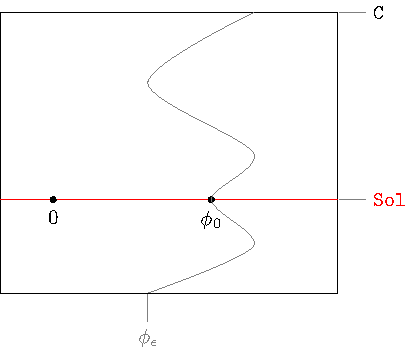
\includegraphics[width=\textwidth]{Pictures/GeometricPicture0}
		\end{minipage}
		\begin{minipage}{0.5\textwidth}
			\begin{itemize}
				\item The set $\Conf$, space of kinematic configurations, is a linear submanifold.\\
					For the sake of simplicity we depict it as a plane, neglecting the complexities related to infinite-dimensional manifods.
				\item Consequently, the space of solutions $ \Sol$ is a linear submanifolds, in our picture a line, containing the section $0$.
			\end{itemize}
		\end{minipage}
		\vspace{1mm}\\
			
		We recall that the main character of the Peierls' procedure are the \emph{Lagrangian densities}, elements in $\Lag(E)$.
		Abstractly, they are maps from kinematic configurations to volume forms on the spacetime. From a more practical point of view we are interested in its twofold nature:
		\begin{itemize}
			\item As the object ruling the dynamics, through the correspondence $\Lagrangian \mapsto Q_\Lagrangian$, or, eventually, as a disturbance on the fixed unperturbed Lagrangian.
			\item As a quantity evaluable on the conformations of the system, through the correspondence  $\Lagrangian \mapsto  \mathcal{O}_\Lagrangian$.
		\end{itemize}
		
		In the first instance, the Peierl's procedure considers a not necessarily linear fixed Lagrangian density $\chi\in \Lag(E)$. The only constraint is imposed on the support condition of $\chi$.\\
		\vspace{1mm}		
		\begin{minipage}{0.5\textwidth}
			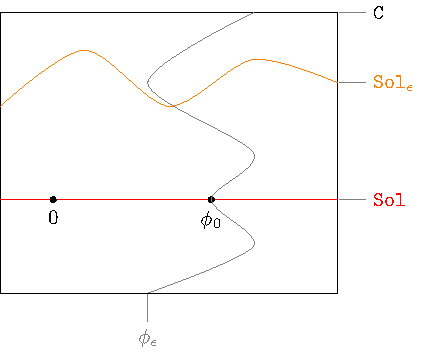
\includegraphics[width=\textwidth]{Pictures/GeometricPicture1}
		\end{minipage}
		\begin{minipage}{0.5\textwidth}
			\begin{itemize}
				\item Call $\Sol_\epsilon$ the space of solutions of the disturbed dynamics equation $Q_{\Lagrangian + \epsilon \chi}$.
					Since $Q_\chi$ is generally not linear we depict this space as an arbitrary curve.\\
					Without any loss of generality we  neglect the possibility that $\Sol \cap \Sol_\epsilon \neq \emptyset$ in this picture.
				\item To an arbitrary variation of a solution $\phi_0$ corresponds a generic parametrized curve on the plane.
			\end{itemize}
		\end{minipage}
		\vspace{1mm}
		\\
		We have proved in Section \ref{Section:PeierlsConstruction} that such choice determines two particular variations of any fixed solution $\phi_0 \in \Sol$.

		\vspace{1mm}		
		\begin{minipage}{0.5\textwidth}
			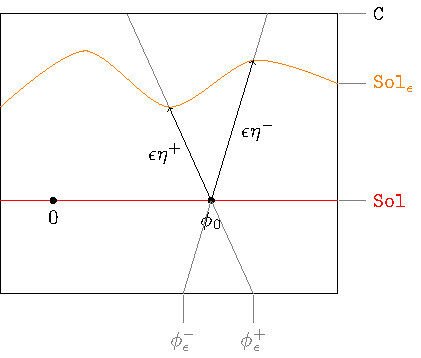
\includegraphics[width=\textwidth]{Pictures/GeometricPicture2}
		\end{minipage}
		\begin{minipage}{0.5\textwidth}
			\begin{itemize}
				\item	Among all the possible linear variations of $\phi_0$, we consider the two variations $$\phi_\epsilon^\pm = \phi_0 + \epsilon \eta_\pm$$ where $\eta_\pm$ are the unique solution of Eq. \ref{PeierlJacobiEqLin}, \textit{i.e.}:
					\begin{displaymath}
   						\eta_\pm = G^\pm \left( - Q_\chi \phi_0 \right)
					\end{displaymath}
					determined by the fixed perturbation $\chi$.
			\end{itemize}
		\end{minipage}
		\vspace{1mm}\\		
	
		In layman terms we can say that the quantity $Q_\chi \phi_0$ quantifies how much $\phi_0$ fails to be a solution of the disturbed equations of motion.
		More explicitly :
		\begin{displaymath}
			P_\epsilon \phi_0 =  \cancel{P \phi_0} + \epsilon Q_\chi \phi_0
		\end{displaymath}
		
		The subsequent step in the Peierls' procedure is the introduction of the effect operator. 
		This object can be seen as a function, associated to the disturbance $\chi$, which maps any continuous fuctional $B$ on $\Conf$ to a functional $\EffectOp_\chi^\pm B$ on $\Sol$. 

		\vspace{1mm}		
		\begin{minipage}{0.5\textwidth}
			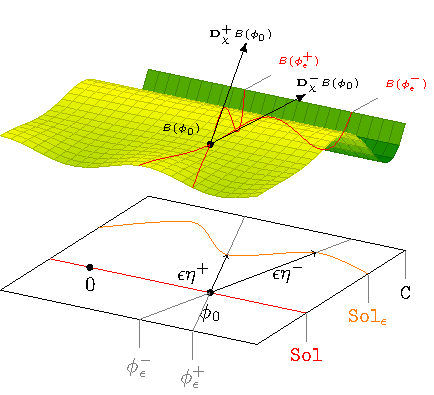
\includegraphics[width=\textwidth]{Pictures/GeometricPicture3}
		\end{minipage}
		\begin{minipage}{0.5\textwidth}
			\begin{itemize}
				\item  A generic continuous functional on the systems can be seen as a continuous function on this $\Real^2$ plane. \\ We depict them as a surface embedded in $\Real^3$.
				\item  Accordingly, $\Sol$ can be regarded as the locus of the  \emph{"total lagrangian"} $  \mathcal{O}_\Lagrangian$ extrema.
				\item	Directly from Definition \ref{EffectOperator} , we can see that $\EffectOp_\chi^\pm B$, the effect of $\chi$ on $B$ evaluated in $\phi_0$, is formally a directional derivative in the direction of $\phi_\epsilon^\pm$ calculated in point $\phi_0$.
					We depict such quantity as a tangent vector to the surface $B$ but, more properly, it corresponds to the value of the inclination of this vector.
			\end{itemize}
		\end{minipage}
		\vspace{1mm}\\	
		All of this machinery has a rather simpler picture when the functional $B$ is linear.

		\vspace{1mm}		
		\begin{minipage}{0.5\textwidth}
			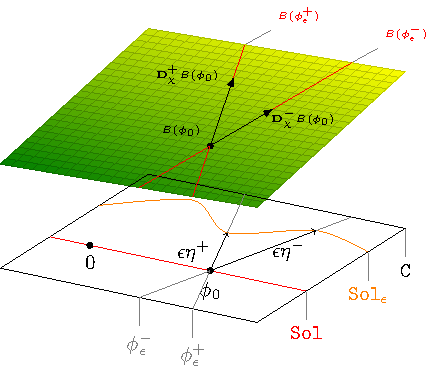
\includegraphics[width=\textwidth]{Pictures/GeometricPictureLinear1}
		\end{minipage}
		\begin{minipage}{0.5\textwidth}
			\begin{itemize}
				\item  When $B$ is a linear functional the effect takes the simple form:
					\begin{displaymath}
						\EffectOp_\chi^\pm B (\phi_0) = B ( \eta_\pm)
					\end{displaymath}
					In this case the dependence on the initial solution $\phi_0$ is accounted implicitly in the construction of perturbation $\eta_\pm(\phi_0)$.
			\end{itemize}
		\end{minipage}
		\vspace{1mm}\\	

		Finally, 
		considering two Lagrangian densities $\chi, \omega$ and the corresponding Lagrangian functional $ \mathcal{O}_\omega$, we achieve the Peierls brackets as:
		\begin{displaymath}
			\{\chi, \omega \}(\phi_0) \coloneqq \EffectOp_\chi^- \mathcal{O}_\omega (\phi_0) - \EffectOp_\chi^+ \mathcal{O}_\omega(\phi_0)
		\end{displaymath}
		According to our \ifToninus (\danger graphical? \danger)\fi geometric picture we can conclude that the Peierls brackets compute the difference between the slopes of the two function $\mathcal{O}_\omega ( \phi_\epsilon^\pm)$, which can be seen as a real function on the single variable $\epsilon$, calculated in $\epsilon=0$.
		We stress again that $ \phi_\epsilon^\pm$ are not arbitrary but they are two specific variations associated to $\chi$ according to the Peierls' procedure.
		
		Thus, the brackets between $\chi$ and $\omega$ vanish in three cases:
		\begin{enumerate}
			\item The two curves $\mathcal{O}_\omega ( \phi_\epsilon^+)$ and $\mathcal{O}_\omega ( \phi_\epsilon^-)$ have the same derivative when evaluated in $\phi_0$.
			\item The starting solution $\phi_0$ is also a solution of $Q_\omega$.\\
				In this case to $\phi_0$ corresponds an extremum of $\mathcal{O}_\omega$ thus its derivative vanishes according to each variation passing trough $\phi_0$.
			\item The starting solution $\phi_0$ is also a solution of $Q_\chi$.\\
				In this case the two perturbation $\phi_\epsilon^\pm$ are degenerate since they correspond to a transformation along a symmetry of the system and $ \eta_\pm = 0$.
		\end{enumerate}
\ifToninus
		\begin{Warning}
			Osservazione colta: nel punto 2 le Peierls sono nulle in quanto sto perturbando lungo una simmetria del sistema ( è qualcosa che ha a che fare con le costanti del moto della perturbazione.
		\end{Warning}
\fi
		
		In conclusion the Peierls brackets compute the quantity:
		\begin{equation}\label{GlobalPeierls}
			\mathcal{O}_\omega ( \phi_{\tiny \epsilon\chi}^+)  - \mathcal{O}_\omega ( \phi_{\tiny \epsilon\chi}^-) \simeq  \{\chi, \omega \}(\phi_0)  + o(\epsilon)
		\end{equation}
		up to the first order, in the \ifToninus "small" \fi expansion parameter $\epsilon$, of a formal Taylor expansion.
		The section $\phi_{\tiny \epsilon\chi}^\pm$ can be seen as the variation of a fixed unperturbed solution $\phi_0$ induced by a perturbation term $\epsilon \chi$ in the Lagrangian ruling the dynamics depending on whether such disturbance propagates forward or backward in time.
		Thus the  quantity \ref{GlobalPeierls} is the difference between the change in the value of the Lagrangian functional $\mathcal{O}_\omega$ evaluated along  the perturbation propagating backward and forward.
		
		\begin{remark}
		The above procedure could be generalized to non linear systems regarding it as a "Linearization".\\
		The plane $\Conf$ depicted above can be seen as a formal tangent space to the non-linear manifold of the kinematic configurations.
		While in the case of linear fields the manifold $\Conf$ is flat and essentially coincides with its unique tangent space, for general field systems  this correspondence can be admitted only locally.
		\end{remark}		
\ifToninus
	\begin{Warning}
				In all of that calculus of variation will assume a pivotal role since the variations could be seen as tangent vectors over the manifold of  kinematic configurations.
	\end{Warning}
\fi	
		
		
		\subsubsection{Peierls brackets role in second quantization.}
		The prequantum structure, in the procedure of quantization via Peierls brackets, requires to restrict ourselves from the set $\Conf$ of all the global sections to the space $\Gamma_0$ of compactly supported sections.

		\vspace{1mm}		
		\begin{minipage}{0.5\textwidth}
			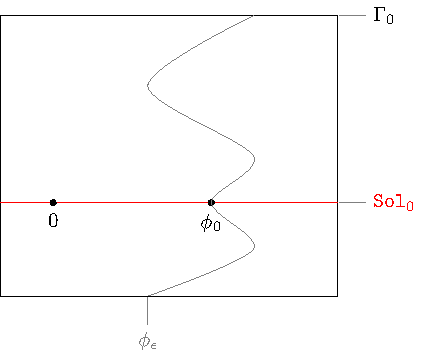
\includegraphics[width=\textwidth]{Pictures/compsupp_GeometricPicture0}
		\end{minipage}
		\begin{minipage}{0.5\textwidth}
			\begin{itemize}
				\item  For linear fields $\Gamma_0$ is still a linear space, we can keep the same representation of the preceding paragraph.
			\end{itemize}
		\end{minipage}
		\vspace{1mm}\\					

	In our picture, the  choice of a pairing 
	\begin{displaymath}
		( \cdot , \cdot ) : \Gamma_0 \times \Gamma_0 \rightarrow \Real^+
	\end{displaymath}
	 ( see Section \ref{Paragraph:Pairing Construction}) corresponds to the attribution of a scalar product on the plane $\Gamma_0$.
	Therefore, $\Gamma_0$ is a vector space rigged with a scalar product $(\cdot , \cdot)$.\\

	To summarize, to each $f\in \Gamma_0$ we associate:
	\begin{enumerate}
		\item a continuous linear functional 
				\footnote{ One should not be misled by the extreme simplification of our geometric visualization.
				It must kept in mind that all the spaces involved are, at best, manifolds with uncountable dimensions.
				Important results as the theorem of Riesz-Fréchet can not be taken in account.}
			on $\Gamma_0$:
			\begin{displaymath}
				F_f(\cdot) = (f, \cdot)
			\end{displaymath}

		\item a Lagrangian density:
			\begin{displaymath}
				f \mapsto \Lagrangian_f \coloneqq \left\langle  f , \cdot \right\rangle_{(x)}
			\end{displaymath}
			where $<\cdot,\cdot>$ is the inner product on the configuration bundle $E$ and such that $F_f \equiv \mathcal{O}_{\Lagrangian_f}$.
		\item a Euler-Lagrange operator:
			\begin{displaymath}
				Q_{f}(\gamma) = - f \qquad \gamma \in \Conf
			\end{displaymath}
			which maps every kinematic configuration to $-f \in \Gamma_0$.
	\end{enumerate}
	In virtue of these correspondences, the Peierls' procedure allows us to equip the space $\Gamma_0$ with a pre-symplectic structure
	\begin{displaymath}
		\tau(f,g) =  \left\lbrace \Lagrangian_f , \Lagrangian_g \right\rbrace = \left( f, (\GreenAdv - \GreenRet) g \right)
	\end{displaymath}
	%
	\vspace{2mm}\\
	Let us visualize this construction in details.
	
		\vspace{1mm}		
		\begin{minipage}{0.5\textwidth}
			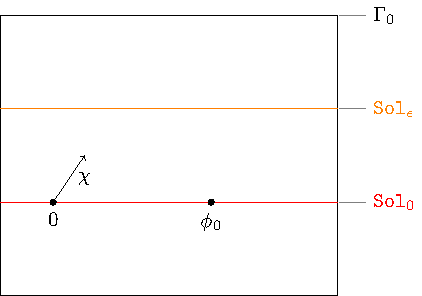
\includegraphics[width=\textwidth]{Pictures/compsupp_GeometricPicture1}
		\end{minipage}
		\begin{minipage}{0.5\textwidth}
			\begin{itemize}
				\item  We are considering only Lagrangian densities constructed from elements of $\Gamma_0$, these can be depicted as vectors on the plane $\Gamma_0$.
				\item 	$\Sol_\epsilon$ consists of all the sections $\gamma \in \Gamma_0$ such that:
					\begin{displaymath}
						P_\epsilon \gamma = ( P  - \epsilon Q_\chi) \gamma = P \gamma - \epsilon \chi = 0
					\end{displaymath}
					They are solutions of the inhomogeneous equation $P \gamma = \epsilon \chi$.
			\end{itemize}
		\end{minipage}
		\vspace{1mm}
		
		Remembering that the solutions of a inhomogeneous differential problem can be built superposing solutions of the homogeneous problem with a "particular solution", 
		we can affirm that
		\begin{displaymath}
			\Sol_\epsilon = \left\lbrace \phi + \epsilon G^\pm \chi \quad \vert \phi \in \Sol \quad  \right\rbrace =
			 \Sol + \epsilon \GreenAdv \chi = \Sol + \epsilon \GreenRet \chi
		\end{displaymath}
		and we can depict this space as a line parallel to $\Sol$.

		
		
		\vspace{1mm}		
		\begin{minipage}{0.5\textwidth}
			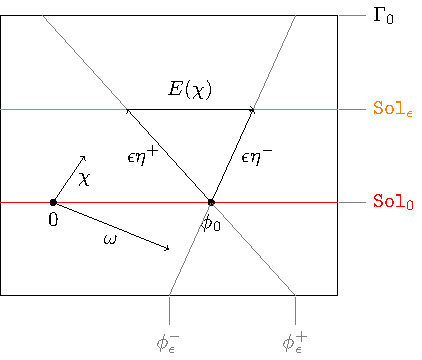
\includegraphics[width=\textwidth]{Pictures/compsupp_GeometricPicture2}
		\end{minipage}
		\begin{minipage}{0.5\textwidth}
			\begin{itemize}
				\item In this case the directions $\eta_\pm$ of the Peierls' variation $\phi_\epsilon^\pm = \phi_0 + \epsilon \eta_\pm$ of a fixed $\phi_0 \in \Sol $ are independent from $\phi_0$:
				\begin{displaymath}
					\eta_\pm = G^\pm (- Q_\chi \phi_0 ) = G^\pm \chi
				\end{displaymath}
				\item consequently $E \chi = (\GreenAdv - \GreenRet) Q_\chi \phi_0$ is always a vector on the line $\Sol_\epsilon \parallel \Sol_0$.\\
				This has been proved in Theorem:	\ref{Teo:IsomorphismBetweenTheTwoSymplectic} through the definition of the isomorphism $\Xi$.
			\end{itemize}
		\end{minipage}
		\vspace{1mm}\\		
	
		The effect of disturbance $\chi$ on an arbitrary continuous linear functional is:
		\begin{displaymath}
			\EffectOp_\chi^\pm B (\phi_0)=B (\eta_\pm) = B ( G^\pm \chi) \qquad \forall \phi_0 \in Sol
		\end{displaymath}		
		Considering instead the Lagrangian functional relative to $\omega \in \Gamma_0$ we find
		\begin{displaymath}
			\EffectOp_\chi^\pm F_\omega (\phi_0) = \left( \omega , G^\pm \chi \right)
		\end{displaymath}
		which leads to the pre-symplectic form $\tau$.
		
		\vspace{1mm}		
		\begin{minipage}{0.5\textwidth}
			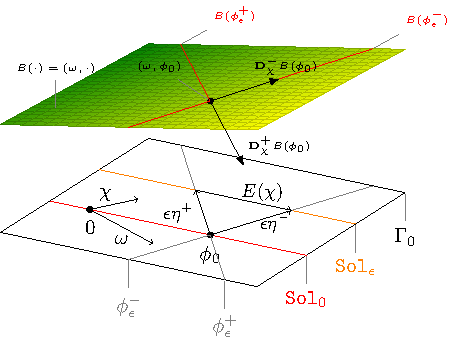
\includegraphics[width=\textwidth]{Pictures/compsupp_GeometricPictureLinear}
		\end{minipage}
		\begin{minipage}{0.5\textwidth}
			\begin{itemize}
				\item For the sake of simplicity we depict the pairing relation as the ordinary inner product  on the plane $\Gamma_0$.
				\item The Lagrangian functional $B_\omega (\cdot) = (\omega, \cdot)$ correspondent to  $\omega \in \Gamma_0$  can be depicted as a plane which intersects plane $ x y$ along the normal to $\omega$.
			\end{itemize}
		\end{minipage}
		\vspace{1mm}\\	
	
		In conclusion, according to our visualization, the brackets between $\chi$ and $\omega$ vanish when:
		\begin{displaymath}
		 \omega \perp E \chi \Longleftrightarrow \chi \perp E \omega
		\end{displaymath}
		where the perpendicularity condition is meant with respect to the inner product on $\Gamma_0$ induced by the pairing \ref{Def:Pairing}.
		
		\vspace{2mm}
		Looking at the picture we can deduce that if $\omega$ is orthogonal to $\Sol_0$ the brackets are necessary null:
			\begin{displaymath}
				 \{\omega, \chi\} = -(E \omega , \chi) = ( \omega , E \chi)=0 \qquad \forall \chi \in \Gamma_0
			\end{displaymath}
		Since $E\omega \in \Sol_0$ the equivalence above is met only if:
		\begin{displaymath}
		(\GreenAdv - \GreenRet) Q_\omega \phi_0= E \omega = 0 
		\end{displaymath}
		This is guaranteed from the condition $\ker(\mathcal{O}_\omega) \supset \Sol$.
		In fact, when the functional $\mathcal{O}_\omega (\cdot) = ( \omega, \cdot): \Conf \rightarrow \Real$ is domain restricted to $\Sol$, it provides degenerate Euler-Lagrange equations: $\left. Q_\omega \right\vert_\Sol = 0$.

\ifToninus
		\begin{Warning}
			Osservando la figura si potrebbe dedurre che 
			\begin{displaymath}
				\omega \perp \Sol_0 \quad \Rightarrow \qquad \{\omega, \chi\} = ( \omega , E \chi)=0 \qquad \forall \chi \in \Gamma_0
			\end{displaymath}
			Ma io ho anche detto che :
			\begin{displaymath}
				E \chi \parallel \Sol_0 \qquad \forall \chi \in \Gamma_0
			\end{displaymath}
			Quindi ho un assurdo
			\begin{displaymath}
				 0 = ( \omega , E \chi)=-( E\omega ,  \chi)\neq 0
			\end{displaymath}
			?\\
			Non necessariamente! 0 è una soluzione e se 
			\begin{displaymath}
				E\omega= 0   \qquad \forall \omega \perp \Sol_0
			\end{displaymath}
			o in altre parole: 
			\begin{displaymath}
				(\omega, \phi) = 0 \quad \forall \phi \in \Sol_0  \qquad \Rightarrow  \quad(\GreenAdv - \GreenRet) Q_\omega \phi_0= 0 
			\end{displaymath}
			Questo è ragionevole perchè il funzionale $\mathcal{O}_\omega (\cdot) = ( \omega, \cdot): \Conf \rightarrow \Real$ se ridotto di domino a $\Sol$ è identicamente nullo ( $\ker(\mathcal{O}_\omega) \supset \Sol$) e  dovrebbe dare $\left. Q_\omega \right\vert_\Sol = 0$.
			\\ non sono sicuro che si possa fare così... 
		\end{Warning}
\fi	
	
		\subsubsection{Peierls Brackets of the Jacobi field}
		Now we take a step further considering the Peierls brackets in the case of a Jacobi Fields.
		\begin{figure}[h!]
			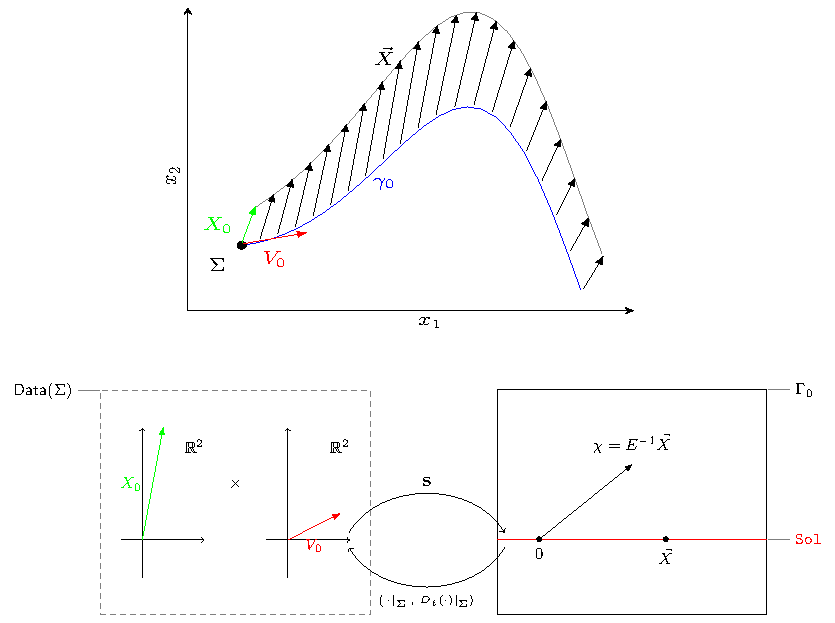
\includegraphics[width=\textwidth]{Pictures/Jacobi_GeometricPicturePanoramica}	
			\caption{ 
			%Impressionistic representation of the Jacobi field system on a  2-dimensional Riemannian manifold $M$.\\
			Below: the geometric structures encoding the "pre-quantum" Jacobi field.
			\\
			Above: a local chart representation of a Jacobi field $\vec{X}$ along a fixed geodesic $\gamma_0$ on a  2-dimensional Riemannian manifold $M$.
			}	
		\end{figure}				

		This example provides a testing ground to compare the two pre-quantization procedures showed in Chapter 3.\\
		The crucial point is that the following correspondences:
		\begin{displaymath}
			(\chi) \in \Gamma_0 \quad \xmapsto{\Xi} \quad (E \chi) \in \Sol \quad \xmapsto{\vert_\Sigma} \quad 
			 \left(\left. E\chi \right\vert_\Sigma , D_t\left.\left( E \chi \right)\right\vert_\Sigma \right) \in\Data(\Sigma)
		\end{displaymath}
		\begin{displaymath}
			 \left(\substack{a\\b}\right) \in\Data(\Sigma) \quad \xmapsto{\SolMap} \quad
			 \left( \SolMap \left(\substack{a\\b}\right) \right)\in \Sol \quad \xmapsto{E^{-1}} \quad 
			 \left( E^{-1}\SolMap \left(\substack{a\\b}\right) \right) \in \Gamma_0
		\end{displaymath}
		are symplectomorphism. This allows us to compare the symplectic form $\tau$ on $\Obs$ with the symplectic form $\Omega$ on $\Data(\Sigma)$.
		
		\vspace{2mm}
		In order to obtain a more intuitive representation we limit ourselves to the most simple case of one-dimensional Riemannian manifolds.

		\vspace{1mm}		
		\begin{minipage}{0.5\textwidth}
			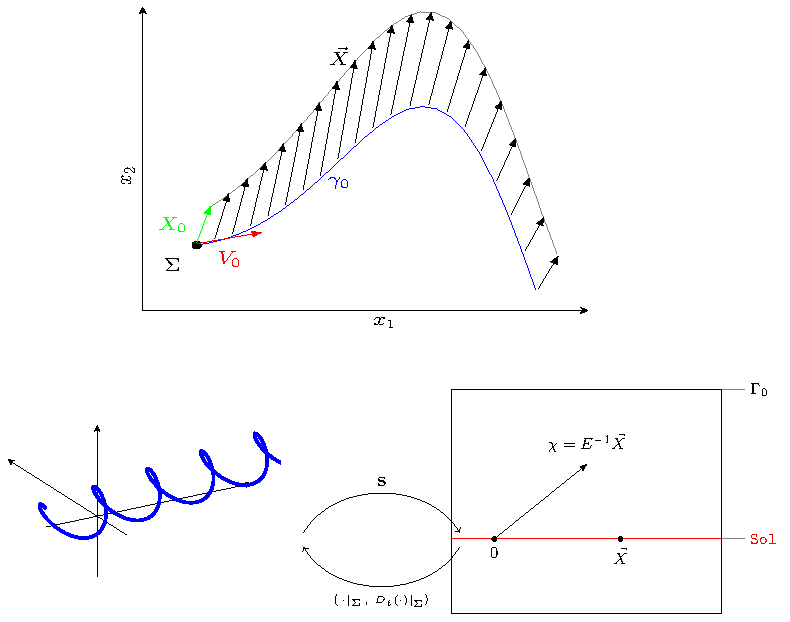
\includegraphics[width=\textwidth]{Pictures/Jacobi1D_GeometricPicture0}
		\end{minipage}
		\begin{minipage}{0.5\textwidth}
			\begin{itemize}
				\item We depict $M$ as an embedded curve in the three dimensional space.
				\item Local charts are simply functions $\Psi: M \rightarrow \Real$, we call $t$ the corresponding coordinate.
				\item Parametrized curves are functions $\gamma: \Real \rightarrow M$, we call $s$ the parameter.
				\item The tangent space to $T_P M$ corresponds to the tangent line to $M$ in $P$.
			\end{itemize}
		\end{minipage}
		\vspace{1mm}\\	
		
		Briefly, to each smooth curve $\gamma$ we associate the ordinary smooth function $f(s) = \Psi \cdot \gamma (s)$.\\
		In this case the metric is simply a smooth, non vanishing, function $g: M \rightarrow \Real$. The inner product between two "tangent vectors" is:
		\begin{displaymath}
			\left< a , b \right> = g a b \qquad \forall a,b \in T_P M \simeq \Real
		\end{displaymath}
		\ifToninus Since it is necessary only a single coordinate ($t$),\fi There is just one Christoffel symbol:
		\begin{displaymath}
			\Gamma^0_{\, 0 0} = \frac{1}{2} g^{-1} \left( \frac{\partial g}{\partial t} \right)
		\end{displaymath}
		The corresponding geodesic equation is:
		\begin{displaymath}
			\partial^2_s \gamma + \frac{1}{2}\left.\left[ g^{-1}  \partial_t g \right] \right\vert_{\gamma(s)}  \left(\partial_s\gamma\right) ^2 = 0
		\end{displaymath}
		Clearly the fields along a fixed geodesic $\gamma(s)$ are scalar functions $X(s) \in \Real$ too.
		Since the Riemann tensor on a one dimensional manifold is null, the single Jacobi equation results:
		\begin{displaymath}
			\partial_s^2 X = 0
		\end{displaymath}
		In conclusion the Jacobi Fields along $\gamma(s)$ are all the straight lines:
		\begin{displaymath}
			X(s) = a + b s
		\end{displaymath}
		therefore $\Sol \simeq \Real^2$ is a two dimensional linear subspace of the linear manifold:
		\begin{displaymath}
			\Gamma_0 = C_0^\infty (\Real) \ifToninus= \{ f: \Real \rightarrow \Real \; \vert \, \textrm{ \tiny smooth, compactly supported}\}\fi
		\end{displaymath}
		From the explicit computation of the Green functions (see Eq. \ref{SimpleGreenFunction}), it follows, moreover, that the exact expression for the Green operators is:
		\begin{displaymath}
			G^\pm \psi (s) = \pm \int_\Real \theta\big(\pm(s-\xi)\big) \left[ s  -\xi\right] \psi(\xi) d\xi
		\end{displaymath}
		for all  $\psi \in \Sigma_0$.
		The effect of the "advanced minus retarded" operator is:
		\begin{displaymath}
			( G^- -  G^+ ) \psi(s) =  -\int_\Real \left[ s -\xi\right] \psi(\xi) d\xi = 
			s \left[-\int_\Real \psi(\xi) d\xi \right] + \left[\int_\Real \xi \psi(\xi) d\xi \right]
		\end{displaymath}
		in agreement with the expected linear expression.
		\ifToninus\begin{Warning}
			I conti  tornano:\\  $E \psi$  è nella forma $(a +b s)$ dunque  è una soluzione.
		\end{Warning}\fi

		\begin{figure}[h!]
			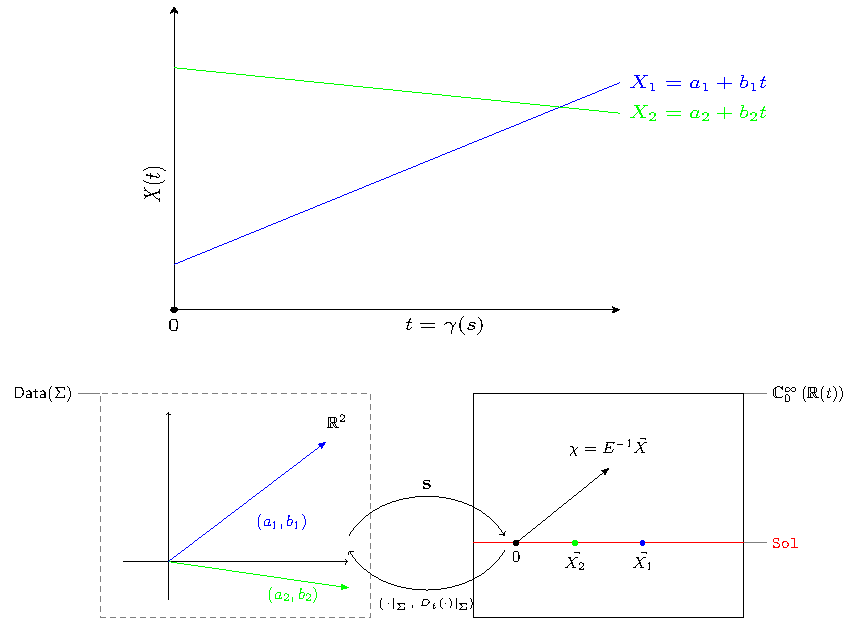
\includegraphics[width=\textwidth]{Pictures/Jacobi1D_GeometricPicturePanoramica}	
			\caption{ 
			%Impressionistic representation of the Jacobi field system on a  2-dimensional Riemannian manifold $M$.\\
			}	
		\end{figure}		


	\subsection{Geometric Mechanics of Classical Fields}
		%-------------------------------------------------------------------------------------------------------------------
		% La scomessa della meccanica Geometrica
		According to Lessing\cite{Lessig2012}, we call "geometric mechanics" the mathematical discipline which employs modern geometry to describe mechanical systems.
		It is no secret that geometry is an intrinsic part of mechanics. For example the space of all admissible configurations of a ordinary mechanical system has the natural geometric structure of a manifold.
		Therefore the bet of geometric mechanics is that is possible to attribute to every mechanical system a  \emph{phase space} together with the implicit claim that it is possible to reconstruct from this space each physically relevant quantity.% relevant to the mechanics. 
		In the spirit of \emph{coordinate-free canonical formalism} the central object, necessary and sufficient, to encode the entire mathematical structure of a classical mechanical system is a \emph{symplectic manifold}.


		%-------------------------------------------------------------------------------------------------------------------
		% Il vantaggio dell'approccio geometrico dal punto di vista degli schemi di quantizzazione
		In view of the quantization schemes this approach has proven to be winning.
		The reason is that from the symplectic structure descends in a simple way a Poisson structure which can be modified in order to encompass the pre-quantum version of the canonical commutation rules.


		%-------------------------------------------------------------------------------------------------------------------
		%Si può fare una meccanica Geometrica per i campi?}	
		Because of the relation of Poisson brackets to quantization, the problem of the quantization of fields required the translation of the canonical formalism from mechanics to field theories (multiple independent variable instead of one).
		One of the most annoying flaws of the usual canonical formalism in field theory is its lack of manifest covariance, that is its lack of explicit invariance under spacetime coordinate transformations (in the context of general relativity). 
			
			This defect is built into the theory from the very beginning, since the usual \emph{Hamiltonian} canonical formalism represents the dynamical variables of classical field theory by functions on some spacelike hypersurface (Cauchy data) and provides differential equations for their time evolution off this hypersurface: 
			it presupposes a splitting of spacetime into space and time, in the form of a foliation of spacetime into Cauchy surfaces.	
			As a result, canonical quantization leads to models of quantum field theory whose covariance is far from obvious and in fact constitutes a formidable problem.
		
		%-------------------------------------------------------------------------------------------------------------------
		%Punto preliminare per realizzare questo progetto è il passaggio dal usual canonical formalism to the "covariant canonical formalism"
		Luckily, the essence of the canonical formalism can be developed in a way that manifestly preserves all the relevant symmetries called "covariant canonical formalism.
		The key ideas are two:
		\begin{itemize}
			\item  for any "sufficently well behaved" system there is a one-to-one correspondence between solutions and initial data.
			\item the point $(q^i,p^i)$ of the phase of an ordinary Hamiltonian system can be seen as initial data of a motion.
						To each point in the phase space it corresponds one and only one direction of the Hamiltonian flow.
		\end{itemize}
		This leads us to the central concept proposed by Crnkovic and Witten\cite{Crnkovic1999}
		
		\begin{definition}
			We call \emph{Covariant Phase Space} of a system the space $( \Sol )$ of all of its solutions to the classical equations of motion,
			in other words the space of classical trajectories of the system. 
		\end{definition}
		
		\begin{example}
			Consider a non-relativistic particle propagating on a Riemannian manifold $X$ with the usual action functional.
			A trajectory is uniquely fixed by the position $x_i \in X$ and the momentum $p\in T^*_x X$ of the particle at a given time, the ordinary Phase space is thus constituted by the pair $(x_i, p_i)$.
			Correspondingly the space of all solutions and hence the (covariant) phase space of the system may be identified with the cotangent bundle $T^*X$ of $X$.
			
			Similarly, the covariant phase space of the relativistic particle on a pseudo-Riemannian manifold X is the space of geodesics of X (in the absence of a background gauge field).
		\end{example}
		Identifying points of the phase space with whole solutions of the equations of motion requires a conceptual shift in thinking about the time development of the system.
		In the standard Hamiltonian framework one identifies solutions of the equations of motion with integral curves of the Hamiltonian vector fields. In the covariant phase space that identification becomes untenable.


		%-------------------------------------------------------------------------------------------------------------------
		%la costruzione fatta con i dati iniziali è simile ma non covariante a vista!
		Since these phase spaces are (locally) naturally parameterized by the suitable boundary conditions or choice of a Cauchy surface (which uniquely determine the corresponding history of the physical system), 
		this construction is strictly related to the pre-symplectic structure proposed in the quantization "by initial data".
		The “covariant” in “covariant phase space” is to indicate that it comes without any particular choice of Cauchy surface.

		%-------------------------------------------------------------------------------------------------------------------
		% Ci sono diverse idee per realizzare questo programma. Il nostro lavoro si inquadra essenzialmente nel "covariant functional formalism" advocated from crinkovic witten
		The hard part is to find a covariant description of a symplectic structure on the covariant Phase Space .
		In the last decades there were many attempts to develop a fully covariant formulation of such object for classical field theories.
		%-------------------------------------------------------------------------------------------------------------------
		% Il nucleo del lavoro come presentato da crinkovic è il covariant phase space. di che si tratta?
		% Ricordare che l'approccio di crinkovic porta alla definizione di una forma simplettica equivalente con quella costruita con il metodo di wald ma covariante.
		% Il metodo di Peierls fornisce una seconda forma di Poisson e l'equivalenza ma tra le due non è ovvia. Khav l'ha provata per sistemi molto generali		
		The “covariant functional formalism”, strongly advocated in the 1980’s by Crnkovic,Witten and Zuckerman,
		is based on the constuction of a symplectic structure starting from a "covariant presymplectic current density"\cite{Crnkovic1999}\cite{Khavkine2014}.
		This approach is slightly different from the construction "by initial data". A glimpse of such construction can be found in Example \ref{Ex:IndipendentPhaseSpace} where we have exhibited a conserved current in order to prove that the symplectic definited in \ref{Def:InitialDataSymplecticForm} is independent from the choice of the Cauchy surface
		% senza scendere nei dettagli bisogna dire che il metodo del cov phase space si basa su un raffinamento del metodo di Wald, è covariantizzazione del metodo sui dati iniziali (notando l'isomorfismo tra dato e soluzione unica)
		% Questo metodo fornisce una forma simplettica sullo spazio delle fasi covarianti allora il metodo di peierls va visto come se fornisse una forma di poisson su ciò che va rivisto come lo spazio degli "osservabili" nel senso di funzione che viene valutata su una configurazione
		% l'equivalenza tra le due stutture l'abbiamo dimostrato per il campo scalare e jacobi sfruttando una corrente conservata.. proprio su un oggetto del genere è definita la costruzione di Crinko vedi crinko e khav	

		\vspace{2mm}
		%-------------------------------------------------------------------------------------------------------------------
		% Come si ricollega tutto ciò a quanto fatto da noi?
		A problem to address is how to frame the Peierls' construction inside the covariant Phase space formalism.
		We have seen in Chapter 2 how the covariant phase space $\Sol$ can be embedded into the space of field configurations $\Conf$.
			This embedding is characterized as the zero locus of the equations of motion. 
			While the bracket $\{\cdot,\cdot\}$ defined by Wald\cite{Wald1994}(see Def \ref{Def:InitialDataSymplecticForm}) and its covariant version on $\Sol$ (see \cite{Khavkine2014}) can be essentially be view as the \emph{symplectic form} of a phase space,
			the Peierls algorithm is a recipe which provide a binary form on the space of Lagrangians.
			Identificating $\Lag$ to the space of the Lagrangian functionals on $\Conf$ is easy to relate the Lagrangian densities to Hamiltonian functions of ordinary mechanics.			
			In this term is more correct to state that the form constructed by the Peierls' algorithm is indeed a non-degenerate Poisson structure on the algebra of functions on the covariant phase space is given by the Peierls bracket.
		
			While symplectic and Poisson structures are obviously related, the two covariant formalisms that we have described naturally appear in somewhat different problems. 
			Only recently has been formalized the equivalence conditions for covariant constructions of the symplectic and Poisson structures in an elegant and fully covariant way, thus without using the canonical formalism as an intermediary \cite{Forger2005}\cite{Khavkine2014}.
				
		%-------------------------------------------------------------------------------------------------------------------
		% Questo argomento è ancora di frontiera per quanto riguarda il rigore matematico complessivo. serve analisi globale per esprimere la geometria differenziale per queste varietà infinito dimensionale
		%nel linguaggio di crnkovic e khavkine si può proporre una formal diffential geometry of the covariant phase space.	
		The main drawback of this geometric point of view is the lack of mathematical rigor, since it is often restricted to the formal extrapolation of techniques from ordinary calculus on manifolds to the infinite dimensional setting.
		Transforming such formal results into mathematical theorems is a separate problem, often highly complex and difficult.
		A further investigation from the mathematical point of view and a serious functional analytical effort are still needed to describe the infinite dimensional spaces of field configurations and algebras of observables using infinite dimensional differential geometry.

		\vspace{2mm}
		%-------------------------------------------------------------------------------------------------------------------
		%In cosa si differenzia il mio lavoro da quello di crinkovic khavkine forger romero?
		% IO ho cercato di fare un espressione generale per il sistema astratto per cui si applica il metodo di Peierls nel modo in cui lo racconta lui ( al netto di strutture di spin, vincoli e gauge)
		% Crnkovic da un espessione generale del metodo dei dati iniziali. La sua costruzione passa per l'identificazione di una corrente conservata (la stessa che io ho esibito nel caso di campo scalare e jacobi per dimostrare l'indipendenza dalla scelta di sigma per il caso di campo scalare (% Lui non parla di peierls!). L'articolo preliminare è fatto assieme a Witten ( nel 300 years of gravitation), esegue questa costruzione in vari casi specifici. 
		
		We want to remark that in the course of this work we focused on the analysis of the steps that make up the Peierls' algorithm.
		It is costumary to refer to the Peierls brackets as the bilinear form $\tau$ acting on $\Obs$ (see Definition \ref{Def:SymplecticTau}) but its original procedure is way more general as it is defined on the whole space of Lagrangian densities, modulo a technical condition on the support.
		
		%-------------------------------------------------------------------------------------------------------------------
		% Disclaimer importante 1: siamo stati sul semplice riguardo i sistemi campo considerati, sono 3 le complicazioni interessanti ad esempio addressate da Khavkine
		In addition, we acknowledge that the abstract take to mechanical systems proposed in Chapter 2 is by no mean the "state of the art"  on the mathematical theory of classical field systems.
		Basically are required three more aspect to be faced in order to present the most general pre-quantum field theory:
		\begin{itemize}
			\item Gauge freedom.
			\item Spin structure.
			\item Constraints.
		\end{itemize}
		An earnest approach to this matters would require an important insight on the mathematical foundations of the classical field systems based on the \emph{Variational Bicomplex}.\cite{G.Sardanashvily2013,Giachetta2009,Khavkine2014}


	\subsection{The quandary of a geometric interpretations}
		%-------------------------------------------------------------------------------------------------------------------
		% Ok, abbiamo visto la pitturizzazione dell'algoritmo di Peierls e inquadrato il ruolo della forma simplettica (x, Ey) costruita a partire da esso all'interno della pittura geometrica della meccanica.
		%questa però non si può dire ontologicamente un'interpretazione geometrica dell'algoritmo
		At this point the reader should have realized that the construction proposed by Peierls' is anything but straightforward.
		It is likely that the author was guided by experience, deducting its general formula from many examples of unequal time Poisson bracket (or rather the quantum commutator) of point fields , computed using the canonical method.
		
		In the course of this section we have provided a geometric visualization of the Peierls construction and identified the role of the corresponding "Poisson form" $(\cdot, E \cdot )$  within the framework of geometric mechanics.
		However this can not be considered by any means a \emph{geometric interpretation}.

				
				
		%-------------------------------------------------------------------------------------------------------------------
		%  Cosa interpretiamo per geometric interpretations che manco o meglio cosa vorremmo fosse un'interpetazione geometrica convincente?
		Despite this both the Peierls' construction and the "initial data" construction (including its covariant version proposed by Crnković) appear quite esoteric and out of the blue.
		Basically these are treated as "black box" which provide a satisfactory symplectic form  from the point of view of quantization schemes.
		They are not justified a priori and each individual steps of both the constructions lack a geometric and physical interpretation.
		
		
		%-------------------------------------------------------------------------------------------------------------------
		%  è da porsi la domanda di cosa ha aggiunto  alla nostra comprensione lo studio del caso del campo di Jacobi
		At this point one could wonders what we have learned to the application of the Peierls method to the Jacobi Fields.
		The main idea was to compare the symplectic form generated by this method by the one constructed trough the initial data method in the particular case of a system with finite dimensional phase space \textit{i.e.} such that the underlying symplectic structure is unique according to the Darboux theorem.

		%-------------------------------------------------------------------------------------------------------------------
		%  Purtroppo non abbiamo trovato un confronto immediato
		Unfortunately, we must note that even in this case the comparison between the two methods is far from being immediate.
%
		%-------------------------------------------------------------------------------------------------------------------
		%  Ciò che può emergere dalla nostra analisi è il ruolo centrale dello spazio geometrico delle lagrangiane che soggiace a tutto il discorso (vs il ruolo maggiore di Dati e soluzione che si ha nel caso di Cov Pha Spa).
		%		Purtroppo si è evidenziato che il confronto dei due metodi non è così immediato come uno potesse sperare in quanto entra in gioco anche la perturbazione nello "spazio delle lagrangiane" la cui interpretazione geometrica non è così diretta. 
		In order to expand the geometrical understanding of Peierls method, we believe would be necessary not only to formalize the mathematical structure of the manifolds $\Data$ and $\Sol$ (which are the basis of the canonical phase space formalism), 
		but in particular has is to be determined the geometric structure of the space of Lagrangian densities which underlies the concept of "disturbance" on which the whole method is based.
\end{document}

